\chapter[Metodologia]{Metodologia}

Neste capítulo, será especificada qual a metodologia de pesquisa científica, dentre as pesquisadas, que mais se adequou ao tema coberto nesse Trabalho de Conclusão de Curso. Posteriormente, são descritos: (i) o planejamento da pesquisa seguido do cronograma que aborda suas atividades, (ii) a metodologia que conduziu o desenvolvimento do simulador em si, e (iii) a metodologia que orientou a análise dos resultados obtidos.

\section{Classificação da pesquisa}

Pesquisas são classificadas de acordo com seus objetivos gerais. O objetivo de uma pesquisa exploratória é a familiarização com o assunto que ainda não foi bem explorado e existem poucas informações acerca do mesmo. Em sua maioria, a pesquisa assume forma de planejamento bibliográfico ou estudo de caso. Essas pesquisas podem envolver levantamento bibliográfico, entrevistas com pessoas que tiveram experiências práticas com o problema pesquisado e também análise de exemplos que estimulem a compreensão \cite{gil}.

Outro tipo de classificação é formulada com base nos procedimentos técnicos utilizados para seu desenvolvimento. A exemplo disto, existe a pesquisa experimental, que se trata de uma pesquisa envolvendo algum tipo de experimento. Consiste ainda em determinar um objeto de estudo, selecionar as variáveis capazes de influenciá-lo e definir as formas de controle e observação dos efeitos que a variável produz no objeto. Sendo assim, as pesquisas experimentais são um procedimento importante para os cientistas testarem hipóteses que estabelecem relações de causa e efeito entre as variáveis. Portanto, essa técnica garante ao pesquisador um caráter de agente ativo e não apenas de mero observador passivo \cite{tafner}.

A pesquisa-ação é um tipo de pesquisa que em oposição ao modelo tradicional pode
ser considerada como “independente” e “objetiva” \cite{rocha}. Segundo \apudonline{thiollent}{rocha}, caracteriza-se com pesquisa-ação:

\begin{citacao}
\begin{normalsize}
"Um tipo de pesquisa social com base empírica, concebida e realizada em estreita associação com uma ação ou com a resolução de um problema coletivo no qual os pesquisadores e os participantes, representativos da situação e/ou do problema, estão envolvidos de forma cooperativa e participativa" \apud{thiollent}{rocha}.
\end{normalsize}
\end{citacao}

Considerando os objetivos de estudo e o referencial bibliográfico levantado até o momento, este projeto se enquadra no modelo de pesquisa exploratório, com análise de resultados baseada em pesquisa-ação.

\section{Planejamento da pesquisa}

O processo de pesquisa foi conduzido inicialmente, por um levantamento bibliográfico, porém, o mesmo foi revisado durante todo o projeto. Durante a fase inicial da pesquisa, algumas atividades tiveram um foco maior, como a definição do escopo, o estudo do domínio e o planejamento da abordagem. Esta última foi executada até o final do desenvolvimento da pesquisa.

Após a fase inicial da pesquisa, algumas outras atividades foram priorizadas, tais como a implementação da prova de conceito, o refinamento da proposta e a elaboração da parte escrita.

As considerações feitas pela banca de TCC 01 foram coletadas e registradas como sugestões de melhoria. A partir dessas sugestões, foram realizadas as devidas alterações no projeto. Com as melhorias implementadas, o desenvolvimento do Simulador Acústico se iniciou e foi conduzido utilizando conceitos de qualidade de código e técnicas de programação estudados durante o curso de graduação em Engenharia de Software.

Ao finalizar o desenvolvimento do Simulador Acústico, os resultados foram coletados e registrados, sendo então incorporados à parte escrita do projeto, que, por sua parte, teve um foco maior na fase final da pesquisa.

Durante esse processo, algumas metodologias de gerência e de desenvolvimento assim como ferramentas e tecnologias que pudessem proporcionar um melhor acompanhamento e suporte ao projeto foram estudadas.

% \section{Modelagem da metodologia}

Com o intuito de ilustrar como se deu a realização e condução deste projeto, segue a figura \ref{modelagem} que apresenta a modelagem do processo metodológico com base na metodologia descrita nesta seção.

\FloatBarrier 
\begin{figure}[!htb]
\centering
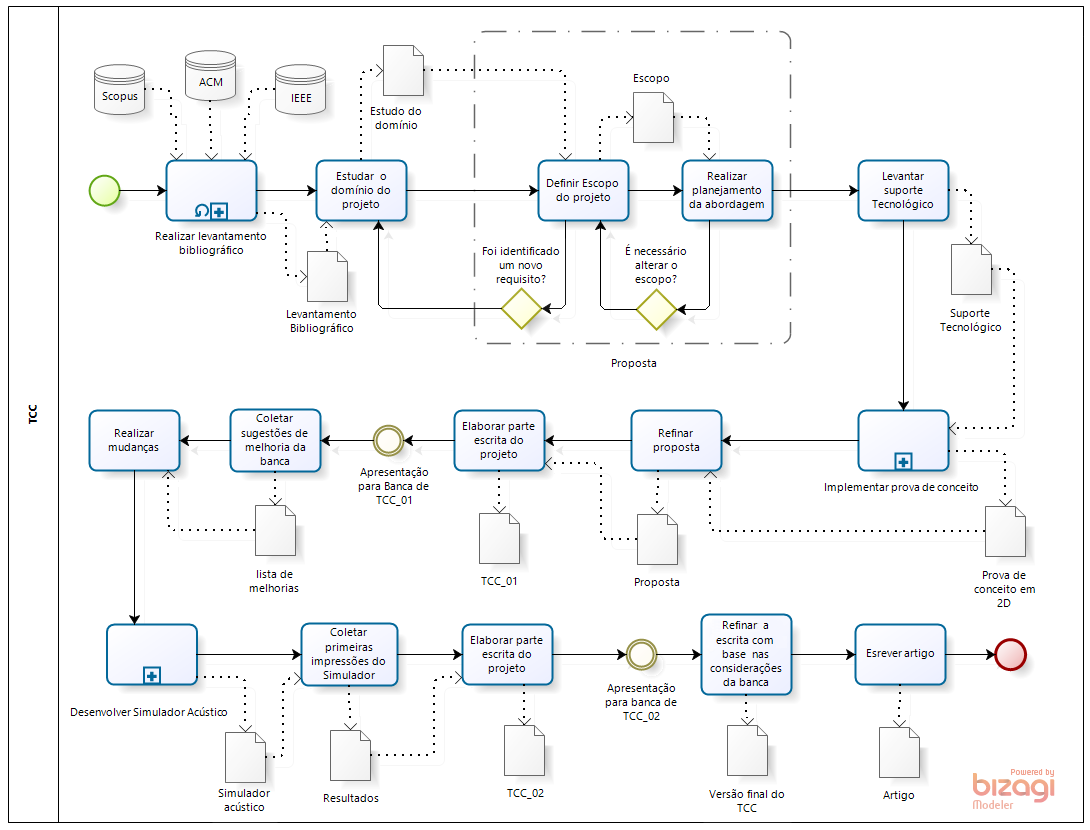
\includegraphics[scale=0.55]{figuras/Processo_TCC}
\caption{Processo TCC}
\label{modelagem}
\end{figure}
%\pagebreak

\section{Cronograma da pesquisa}

Segue o cronograma nas tabelas \ref{tabela_tcc1} e \ref{tabela_tcc2} visando demonstrar como as principais atividades foram conduzidas ao longo deste trabalho.

\begin{center}
%\begin{table}[!htb]
%\centering
\begin{longtable}{l|c|c|c|c|c}

& Ago & Set & Out & Nov & Dez\\ \hline
\endfirsthead

\multicolumn{6}{c}
{{\bfseries \tablename\ \thetable{} -- Continuação da página anterior}} \\
& Ago & Set & Out & Nov & Dez\\ \hline 
\endhead
%\hline 
\multicolumn{6}{c}{{Continua na página seguinte}} \\ %\hline
\endfoot
\endlastfoot

Realizar levantamento bibliográfico 		& X & X & X &   &   \\ \hline
Estudar domínio do projeto 				& X &   &   &   &   \\ \hline
Definir escopo do projeto        		& X & X &   &   &   \\ \hline
Realizar planejamento da abordagem 		& X & X &   &   &   \\ \hline
Levantar suporte tecnológico 			& X & X &   &   &   \\ \hline
Implementar da prova de conceito 		&   & X &   &   &   \\ \hline
Refinar proposta 						&   &   & X &   &   \\ \hline
Elaborar parte escrita do projeto 		&   & X & X &   &   \\ \hline
Apresentação para a Banca de TCC 1 		&   &   &   & X &   \\ \hline
Coletar sugestões de melhoria da banca  	&   &   &   & X &   \\ \hline
Realizar mudanças  						&   &   &   &   & X \\ \hline

%\end{longtable}
\caption{Cronograma TCC 1 (2014)}
\label{tabela_tcc1}
\end{longtable}
\end{center}

\begin{center}
%\begin{table}[!htb]
%\centering
\begin{longtable}{p{7cm}|c|c|c|c|c|c|c}

& Jun & Jul & Ago & Set & Out & Nov & Dez \\ \hline
\endfirsthead

\multicolumn{8}{c}
{{\bfseries \tablename\ \thetable{} -- Continuação da página anterior}} \\
& Jun & Jul & Ago & Set & Out & Nov & Dez \\ \hline
\endhead
%\hline 
\multicolumn{8}{c}{{Continua na página seguinte}} \\ %\hline
\endfoot
\endlastfoot

Desenvolver simulador acústico								&X&X&X& & & &  \\ \hline
Coletar primeiras impressões do simulador 					& & & &X& & &  \\ \hline
Elaborar parte escrita do projeto		 					& & & & &X& &  \\ \hline
Apresentação para a Banca de TCC 2 							& & & & & &X&  \\ \hline
Refinar a escrita com base nas considerações da Banca 		& & & & & &X&  \\ \hline
Escrever Artigo 												& & & & & & &X \\ \hline

%\end{longtable}
\caption{Cronograma TCC 2 (2015)}
\label{tabela_tcc2}
\end{longtable}
\end{center}

%\pagebreak
%\clearpage
%\newpage
%\FloatBarrier 

\section{Metodologia adotada no desenvolvimento do simulador}

Scrum\footnote{\url{https://www.scrum.org/}} é uma estrutura de processo que tem sido usado para gerenciar o desenvolvimento de produtos complexos desde o início da década de 1990. Scrum não é um processo ou uma técnica para a construção de produtos, o Scrum é um quadro no qual você pode empregar diversos processos e técnicas. Scrum deixa clara a eficácia relativa das suas práticas de gestão de desenvolvimento de produto e de modo que você pode melhorar \cite{schwaber}.

O desenvolvimento do simulador proposto neste trabalho foi conduzido considerando o modelo interativo incremental, onde foram realizadas algumas adaptações na metodologia ágil de desenvolvimento Scrum, figura \ref{scrum_adaptado}. Para este projeto, foram definidas sprints com duração de uma semana.

\FloatBarrier 
\begin{figure}[!htb]
\centering
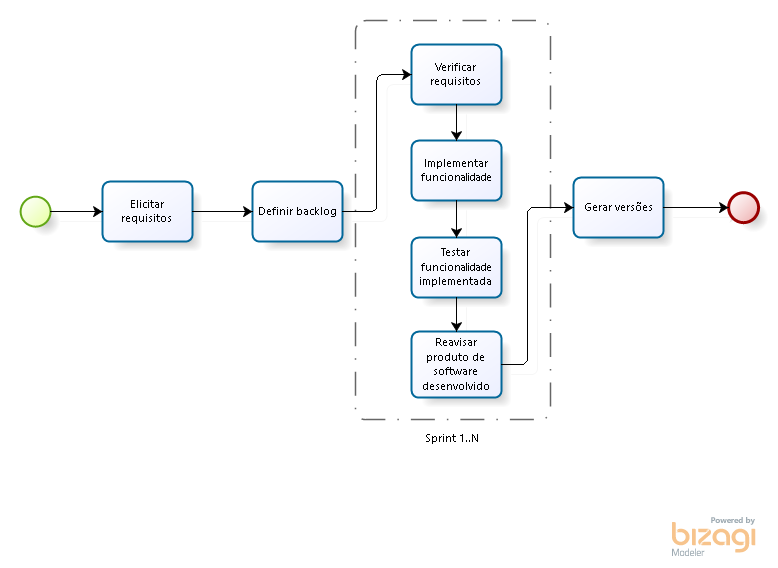
\includegraphics[scale=0.7]{figuras/scrum_adaptado}
\caption{Adaptação do Scrum para este TCC}
\label{scrum_adaptado}
\end{figure}

Para a elicitação dos requisitos, foram levantadas histórias de usuário baseadas nos conceitos de acústica arquitetônica abordados no referencial teórico, assim como os conhecimentos adquiridos ao longo das disciplinas do curso de graduação em Engenharia de Software. O product backlog inicial deste trabalho está representado na tabela \ref{backlog_inicial}. Vale ressaltar que ocorreram algumas modificações durante o processo de desenvolvimento do simulador, assim como é previsto no Scrum.

\begin{table}[!htb]
\centering
\begin{tabular}{|p{4cm}|p{10cm}|}\hline
Identificador & História de usuário\\ \hline
US01 & Como engenheiro, gostaria de definir as configurações de um ambiente tridimensional onde serão realizadas as simulações.\\ \hline
US02 & Como engenheiro, gostaria de definir obstáculos dentro do ambiente de simulação assim como seus respectivos índices de absorção. \\ \hline
US03 & Como engenheiro, gostaria de configurar uma fonte sonora e posicioná-la dentro do ambiente de simulação.\\ \hline
US04 & Como engenheiro, gostaria de poder iniciar, pausar, retomar e parar uma simulação a qualquer momento após a configuração dos obstáculos e da fonte sonora. \\ \hline
US05 & Como engenheiro, gostaria de poder remover um obstáculo ou fonte sonora da simulação.\\ \hline
US06 & Como engenheiro, gostaria de poder definir a velocidade da simulação. \\ \hline
US07 & Como engenheiro, gostaria de poder acompanhar o comportamento do som dentro do ambiente especificado durante a simulação.\\ \hline
US08 & Como engenheiro, gostaria de acompanhar o nível de intensidade sonora dentro da sala durante a simulação.\\ \hline
US09 & Como engenheiro, gostaria de saber qual foi o tempo de reverberação ao fim da simulação.\\ \hline
US10 & Como engenheiro, quero um agente capaz de representar o som dentro de um ambiente fechado considerando sua propagação e suas reflexões.\\ \hline

\end{tabular}
\caption{Product Backlog Inicial}\label{backlog_inicial}
\end{table}

Durante a execução deste trabalho, foi percebido que o uso de uma interface gráfica que pudesse auxiliar na configuração do ambiente assim como no controle e na visualização da simulação, poderia ser útil para nortear as atividades de desenvolvimento e tornar o simulador passível de uso a um usuário final, o que não era possível apenas com a máquina de raciocínio do simulador implementada. 

Como a implementação da interface gráfica não estava prevista no planejamento inicial deste trabalho, foi preciso reduzir o escopo para conseguir completar essa atividade. Sendo assim, algumas alterações no product backlog inicial do projeto foram realizadas. Dentre essas alterações temos a modificação da US01: \textit{"Como engenheiro, gostaria de definir as configurações de um ambiente tridimensional onde serão realizadas as simulações"}. O escopo dessa história foi reduzido, permitindo apenas a configuração de um ambiente bidimensional.

Também foi adicionada uma nova história para a implementação da interface gráfica com o usuário, onde será possível configurar, controlar e visualizar a simulação.

O product backlog final desse projeto pode ser visto na tabela \ref{backlog_final}.

\begin{table}[!htb]
\centering
\begin{tabular}{|p{4cm}|p{10cm}|}\hline
Identificador & História de usuário\\ \hline
US01 & Como engenheiro, gostaria de definir as configurações de um ambiente bidimensional onde serão realizadas as simulações.\\ \hline
US02 & Como engenheiro, gostaria de definir obstáculos dentro do ambiente de simulação assim como seus respectivos índices de absorção.\\ \hline
US03 & Como engenheiro, gostaria de configurar uma fonte sonora e posicioná-la dentro do ambiente de simulação.\\ \hline
US04 & Como engenheiro, gostaria de poder iniciar, pausar, retomar e parar uma simulação a qualquer momento após a configuração dos obstáculos e da fonte sonora. \\ \hline
US05 & Como engenheiro, gostaria de poder remover um obstáculo ou fonte sonora da simulação.\\ \hline
US06 & Como engenheiro, gostaria de poder definir a velocidade da simulação. \\ \hline
US07 & Como engenheiro, gostaria de poder acompanhar o comportamento do som dentro do ambiente especificado durante a simulação. \\ \hline
US08 & Como engenheiro, gostaria de acompanhar o nível de intensidade sonora dentro da sala durante a simulação. \\ \hline
US09 & Como engenheiro, gostaria de saber qual foi o tempo de reverberação ao fim da simulação. \\ \hline
US10 & Como engenheiro, quero um agente capaz de representar o som dentro de um ambiente fechado considerando sua propagação e suas reflexões. \\ \hline
US11 & Como engenheiro, gostaria de poder configurar, controlar e visualizar minha simulação por meio de uma interface gráfica. \\ \hline

\end{tabular}
\caption{Product Backlog Final}\label{backlog_final}
\end{table}

Cada história foi dividia em tarefas antes de se iniciar sua implementação, essas tarefas foram úteis para entender melhor o problema e auxiliar a estimar a sua complexidade em relação ao seu desenvolvimento.

As tarefas relacionadas a cada história foram:

\textbf{US01:} Como engenheiro, gostaria de definir as configurações de um ambiente bidimensional onde serão realizadas as simulações.

\begin{itemize}
\item Implementar agente que irá controlar o ambiente de simulação.
\item Implementar rotina para definição das dimensões do ambiente.
\end{itemize}

\textbf{US02:} Como engenheiro, gostaria de definir obstáculos dentro do ambiente de simulação assim como seus respectivos índices de absorção.

\begin{itemize}
\item Implementar classe Obstaculo.
\item Implementar rotina para adição de obstáculos dentro do ambiente.
\item Implementar rotina para configurar os parâmetros dos obstáculos, tais como dimenções, localização e índices de absorção.
\end{itemize}

\textbf{US03:} Como engenheiro, gostaria de configurar uma fonte sonora e posicioná-la dentro do ambiente de simulação.

\begin{itemize}
\item Implementar agente responsável por representar uma fonte sonora dentro do ambiente.
\item Implementar comunicação entre os agentes Ambiente e FonteSonora.
\item Implementar rotina para emissão do pulso sonoro.
\end{itemize}
	
\textbf{US04:} Como engenheiro, gostaria de poder iniciar, pausar, retomar e parar uma simulação a qualquer momento após a configuração dos obstáculos e da fonte sonora.

\begin{itemize}
\item Implementar rotina para a verificação da existência obstáculos e fonte sonora.
\item Implementar rotina de verificação de status da simulação (em execução, parada ou encerrada).
\item Implementar rotina de execução da simulação.
\item Implementar rotina de pausa da simulação em andamento.
\item Implementar rotina para retomar uma simulação pausada.
\item Implementar rotina para encerrar uma simulação.
\end{itemize}
	
\textbf{US05:} Como engenheiro, gostaria de poder remover um obstáculo ou fonte sonora da simulação.

\begin{itemize}
\item Implementar rotina de remoção de um obstáculo dentro do ambiente.
\item Implementar rotina de remoção de uma fonte sonora dentro do ambiente.
\end{itemize}
	
\textbf{US06:} Como engenheiro, gostaria de poder definir a velocidade da simulação.

\begin{itemize}
\item Implementar rotina de configuração da velocidade da simulação.
\item Implementar rotina de verificação da velocidade da simulação pelo agente sonoro.
\item Implementar rotina de cálculo do tamanho do passo por tempo de atualização do agente sonoro.
\end{itemize}
	
\textbf{US07:} Como engenheiro, gostaria de poder acompanhar o comportamento do som dentro do ambiente especificado durante a simulação.

\begin{itemize}
\item Implementar rotina de atualização dos parâmetros do agente sonoro a serem acompanhados.
\item Implementar rotina de monitoramento dos parâmetros de cada agente sonoro presente no ambiente durante a simulação.
\item Implementar rotina de renderização da interface gráfica com o usuário.
\end{itemize}
	
\textbf{US08:} Como engenheiro, gostaria de acompanhar o nível de intensidade sonora dentro da sala durante a simulação.

\begin{itemize}
\item Implementar rotina de leitura dos níveis de intensidade sonora de cada som dentro do ambiente.
\item Implementar rotina de cálculo de nível de intensidade sonora total dentro do ambiente.
\item Implementar rotina de monitoramento do nível de intensidade sonora total dentro do ambiente.
\end{itemize}
	
\textbf{US09:} Como engenheiro, gostaria de saber qual foi o tempo de reverberação ao fim da simulação.

\begin{itemize}
\item Implementar critério de parada da simulação com base na diminuição em 60dB do nível de intensidade sonora inicial da simulação.
\item Implementar rotina de cálculo do tempo de simulação com base na distância percorrida pelos agentes sonoros.
\item Implementar rotina de cálculo do tempo de reverberação baseado no critério de parada da simulação.
\item Implementar rotina de monitoramento do tempo de reverberação dentro do ambiente.
\end{itemize}
	
\textbf{US10:} Como engenheiro, quero um agente capaz de representar o som dentro de um ambiente fechado considerando sua propagação e suas reflexões.

\begin{itemize}
\item Implementar agente Sonoro.
\item Implementar comunicação entre o agente sonoro e sua fonte sonora.
\item Implementar rotinas de cálculo da propagação sonora.
\item Implementar rotinas de identificação de obstáculos dentro do ambiente.
\item Implementar rotinas de colisão do agente sonoro com obstáculos dentro do ambiente.
\item Implementar rotinas de reflexão sonora.
\end{itemize}
	
\textbf{US11:} Como engenheiro, gostaria de poder configurar, controlar e visualizar minha simulação por meio de uma interface gráfica.

\begin{itemize}
\item Implementar interface com o usuário.
\item Implementar recursos de visualização gráfica da simulação.
\end{itemize}

No Roadmap da tabela \ref{cronograma_sprints}, é possível visualizar quais atividades foram realizadas em cada sprint, assim como suas respectivas datas de início e de término. Durante o desenvolvimento do simulador, foram dedicadas algumas sprints para atividades de refatoração do código fonte.

\begin{table}[!htb]
\centering
\caption{Roadmap}
\label{cronograma_sprints}
\begin{tabular}{|l|l|l|l|}
\hline
Sprint    & Atividade        			& Data de início & Data de Término \\ \hline
Sprint 1  & Implementar US01 			& 07/06/2015     & 14/06/2015      \\ \hline
Sprint 2  & Implementar US02 			& 14/06/2015     & 21/06/2015      \\ \hline
Sprint 3  & Implementar US03 			& 21/06/2015     & 28/07/2015      \\ \hline
Sprint 4  & Implementar US10 			& 28/06/2015     & 05/07/2015      \\ \hline
Sprint 5  & Implementar US05 			& 05/07/2015     & 12/07/2015      \\ \hline
Sprint 6  & Implementar US04 			& 12/07/2015     & 19/07/2015      \\ \hline
Sprint 7  & Atividade de Refatoração		& 19/07/2015	 	 & 26/07/2015	  \\ \hline
Sprint 8  & Implementar US06 			& 26/07/2015     & 02/08/2015      \\ \hline
Sprint 9  & Implementar US11 			& 02/08/2015     & 09/08/2015      \\ \hline
Sprint 10 & Implementar US07 			& 09/08/2015     & 16/08/2015      \\ \hline
Sprint 11 & Implementar US08 			& 16/08/2015     & 23/08/2015      \\ \hline
Sprint 12 & Implementar US09 			& 23/08/2015     & 30/08/2015      \\ \hline
Sprint 13 & Atividade de Refatoração		& 30/08/2015     & 06/09/2015	   \\ \hline
\end{tabular}
\end{table}

A tabela \ref{backlog_conclusao} apresenta o percentual de conclusão das tarefas de cada história de usuário presente no Backlog final deste simulador.

\begin{center}
%\begin{table}[htbp]
%\centering
\begin{longtable}{|c|p{11.5cm}|l|}
\caption{Percentual de conclusão das tarefas}
\label{backlog_conclusao}\\
%\begin{tabular}{|c|p{10cm}|l|}
\hline
Estória             & Tarefa                                                                                                                          & Percentual \\ \hline
\endfirsthead

\multicolumn{3}{c}
{{\bfseries \tablename\ \thetable{} -- Continuação da página anterior}} \\
\hline Estória &
Tarefa &
Percentual \\ \hline 
\endhead
%\hline 
\multicolumn{3}{r}{{Continua na página seguinte}} \\ %\hline
\endfoot
\endlastfoot

\multirow{2}{*}{01} & Implementar agente que irá controlar o ambiente de simulação.                                                                   & 100\%      \\ \cline{2-3} 
                    & Implementar rotina para definição das dimensões do ambiente.                                                                    & 100\%      \\ \hline
\multirow{3}{*}{02} & Implementar classe Obstaculo.                                                                                                   & 100\%      \\ \cline{2-3} 
                    & Implementar rotina para adição de obstáculos dentro do ambiente.                                                                & 100\%      \\ \cline{2-3} 
                    & Implementar rotina para configurar os parâmetros dos obstáculos, tais como dimenções, localização e índices de absorção.        & 100\%      \\ \hline
\multirow{3}{*}{03} & Implementar agente responsável por representar uma fonte sonora dentro do ambiente.                                             & 100\%      \\ \cline{2-3} 
                    & Implementar comunicação entre os agentes Ambiente e FonteSonora.                                                                & 100\%      \\ \cline{2-3} 
                    & Implementar rotina para emissão do pulso sonoro.                                                                                & 100\%      \\ \hline
\multirow{6}{*}{04} & Implementar rotina para a verificação da existência obstáculos e fonte sonora.                                                  & 100\%      \\ \cline{2-3} 
                    & Implementar rotina de verificação de status da simulação (em execução, parada ou encerrada).                                    & 100\%      \\ \cline{2-3} 
                    & Implementar rotina de execução da simulação.                                                                                    & 100\%      \\ \cline{2-3} 
                    & Implementar rotina de pausa da simulação em andamento.                                                                          & 100\%      \\ \cline{2-3} 
                    & Implementar rotina para retomar uma simulação pausada.                                                                          & 100\%      \\ \cline{2-3} 
                    & Implementar rotina para encerrar uma simulação.                                                                                 & 100\%      \\ \hline
\multirow{2}{*}{05} & Implementar rotina de remoção de um obstáculo dentro do ambiente.                                                               & 100\%      \\ \cline{2-3} 
                    & \begin{tabular}[c]{@{}l@{}}Implementar rotina de remoção de uma fonte sonora dentro do \\ ambiente.\end{tabular}                & 100\%      \\ \hline
\multirow{3}{*}{06} & Implementar rotina de configuração da velocidade da simulação.                                                                  & 100\%      \\ \cline{2-3} 
                    & Implementar rotina de verificação da velocidade da simulação pelo agente sonoro.                                                & 100\%      \\ \cline{2-3} 
                    & Implementar rotina de cálculo do tamanho do passo por tempo de atualização do agente sonoro.                                    & 100\%      \\ \hline
\multirow{3}{*}{07} & Implementar rotina de atualização dos parâmetros do agente sonoro a serem acompanhados.                                         & 100\%      \\ \cline{2-3} 
                    & Implementar rotina de monitoramento dos parâmetros de cada agente sonoro presente no ambiente durante a simulação.              & 100\%      \\ \cline{2-3} 
                    & Implementar rotina de renderização da interface gráfica com o usuário.                                                          & 100\%      \\ \hline
\multirow{3}{*}{08} & Implementar rotina de leitura dos níveis de intensidade sonora de cada som dentro do ambiente.                                  & 100\%      \\ \cline{2-3} 
                    & Implementar rotina de cálculo de nível de intensidade sonora total dentro do ambiente.                                          & 100\%      \\ \cline{2-3} 
                    & Implementar rotina de monitoramento do nível de intensidade sonora total dentro do ambiente.                                    & 100\%      \\ \hline
\multirow{4}{*}{09} & Implementar critério de parada da simulação com base na diminuição em 60dB do nível de intensidade sonora inicial da simulação. & 100\%      \\ \cline{2-3} 
                    & Implementar rotina de cálculo do tempo de simulação com base na distância percorrida pelos agentes sonoros.                     & 100\%      \\ \cline{2-3} 
                    & Implementar rotina de cálculo do tempo de reverberação baseado no critério de parada da simulação.                              & 100\%      \\ \cline{2-3} 
                    & Implementar rotina de monitoramento do tempo de reverberação dentro do ambiente.                                                & 100\%      \\ \hline
\multirow{6}{*}{10} & Implementar agente Sonoro.                                                                                                      & 100\%      \\ \cline{2-3} 
                    & Implementar comunicação entre o agente sonoro e sua fonte sonora.                                                               & 100\%      \\ \cline{2-3} 
                    & Implementar rotinas de cálculo da propagação sonora.                                                                            & 100\%      \\ \cline{2-3} 
                    & Implementar rotinas de identificação de obstáculos dentro do ambiente.                                                          & 100\%      \\ \cline{2-3} 
                    & Implementar rotinas de colisão do agente sonoro com obstáculos dentro do ambiente.                                              & 100\%      \\ \cline{2-3} 
                    & Implementar rotinas de reflexão sonora.                                                                                         & 100\%      \\ \hline
\multirow{2}{*}{11} & Implementar interface com o usuário.                                                                                            & 100\%      \\ \cline{2-3} 
                    & Implementar recursos de visualização gráfica da simulação.                                                                      & 100\%      \\ \hline
%\end{tabular}
%\end{table}
\end{longtable}
\end{center}


\section{Metodologia adotada na análise dos resultados}

Cenário de Uso tem sua origem, enquanto "modalidade de pesquisa", em outros contextos, tais como estudos de mercado e modelos estratégicos \cite{tonicenarios}. 

Outro tópico existente sobre Cenários de Uso, no contexto da computação, é dentro do escopo de Casos de Uso. Nesse caso, apesar de existirem semelhanças entre os Cenários de Uso como algo complementar às modalidades de pesquisa conhecidas e Cenários de Uso no contexto de Caso de Uso, foge da noção desejada para o objetivo neste trabalho \cite{rezende}.

Para a análise dos resultados neste trabalho, foi utilizada uma abordagem baseada em pesquisa-ação combinada com cenário de uso. O objetivo é identificar  problemas relevantes  em cenários de uso especificamente desenhados para testes no simulador. Esses cenários compreenderão descritivos em termos de hardware, configuração, questões atendidas, resultados obtidos e ações realizadas em termos de refinamento.

\section{Considerações finais}

Este trabalho consiste consiste no desenvolvimento de um simulador acústico, baseado em sistemas multiagentes, onde os sons são representados como agentes autônomos dentro do ambiente, sendo capazes de interagir com outros sons e com os recursos presentes no ambiente através da troca de mensagens e de forma assíncrona. Trata-se de uma pesquisa exploratória, cujos resultados foram analisados via pesquisa-ação.

A fim de refinar a proposta inicial do trabalho, que antes era baseada apenas no referencial teórico estudado, foi desenvolvida uma prova de conceito, onde foi criada uma representação bidimensional de um ambiente, com obstáculos e seus respectivos coeficientes de absorção, fontes sonoras e um conjunto de sons percorrendo e interagindo com os elementos presentes no sistema.

Com a implementação da prova de conceito foi possível identificar alguns problemas de desempenho que puderam ser reduzidos com um modelo de solução multiparadigma. O uso dos paradigmas orientado a objetos e multiagentes, além de melhorar o desempenho do sistema implementado na prova de conceito, tornou o modelo mais claro, sendo mais intuitiva a representação de obstáculos como objetos de software.

Uma proposta refinada do simulador acústico foi elaborada ao final desse processo metodológico a partir das evidências observadas com a prova de conceito, bem como de ciclos iterativos de pesquisa-ação. Como resultado final tem-se o modelo escrito deste capítulo.